\documentclass[11pt]{article}
\usepackage[utf8]{inputenc}\usepackage[T1]{fontenc}
\usepackage{amsmath,amssymb,amsthm}\usepackage[margin=1in]{geometry}
\usepackage{graphicx}\usepackage{booktabs}
\usepackage[hidelinks]{hyperref}
\newtheorem{observation}{Observation}

\title{The Semiprime Neighbour on the $6N$ Skeleton:\\
A Slower $\omega$-Enrichment and Its Mechanism}
\author{Ruqing Chen\\
\small GUT Geoservice Inc., Montreal, Quebec, Canada\\
\small \texttt{ruqing@hotmail.com}}
\date{\today}

\begin{document}
\maketitle

\begin{abstract}
Part~XII established that twin centres enrich with the factor count
$\omega_{>3}(N)$ through the single-prime law $P(q\mid N\mid\text{twin})=1/(q-2)$.
Here we relax the right member from prime to \emph{prime-or-semiprime}: we count
centres with $6N-1$ prime and $6N+1$ either prime or a product of exactly two
primes. This neighbour count also enriches with $\omega_{>3}(N)$, but
systematically \emph{more slowly} than the twin: on $S_9$ ($3.5\times10^6$ centres
with $6N-1$ prime at $\omega=1$), the twin rate rises to $1.81\times$ at $\omega=5$
while the exactly-semiprime part rises only to $1.37\times$. We give the mechanism:
the small-prime avoidance that a factor-rich $N$ imposes on $6N+1$ helps a prime
(all-or-nothing) more than a semiprime (which may carry one small factor), and we
confirm it directly---among semiprime $6N+1$, the fraction with a prime factor
$\le97$ falls from $0.56$ at $\omega=1$ to $0.41$ at $\omega=5$, so factor-rich $N$
pushes $6N+1$ toward large$\times$large semiprimes. The local densities are the
classical Hardy--Littlewood/Landau type; the contribution is the measured slower
enrichment and its factor-structure mechanism. An exact double-factor CRT closed
form is left open, as the semiprime's two-factor structure does not reduce to the
clean single-prime $1/(q-2)$ of the twin. No claim is made about the infinitude of
any pattern.
\end{abstract}

\section{The relaxed neighbour}

The twin counts centres $N$ with both wings $6N\pm1$ prime; Part~XII showed the
count enriches with $\omega_{>3}(N)$ via $P(q\mid N\mid\text{twin})=1/(q-2)$. We
relax the right wing: keep $6N-1$ prime, but allow $6N+1$ to be \emph{prime or
semiprime}, where a semiprime is a product of exactly two primes (with
multiplicity, e.g.\ $25=5^2$, $35=5\cdot7$), i.e.\ $\Omega(6N+1)\in\{1,2\}$ with
$\Omega$ the prime-factor count with multiplicity. This is the natural
``Chen-type'' relaxation of the twin condition, and we ask how its conditional
density depends on $\omega_{>3}(N)$.

\section{A slower enrichment}

Binned by $\omega_{>3}(N)$ and normalised to $\omega=1$ (Table~\ref{tab:enr},
Fig.~\ref{fig:semi} left), all three rates rise with $\omega$, but at different
speeds. Decomposing the relaxed rate into its prime part (the twin) and its
exactly-semiprime part ($\Omega(6N+1)=2$):

\begin{table}[h]\centering\small
\begin{tabular}{rrccc}
\toprule
$\omega$ & $\#(6N{-}1\text{ pr})$ & twin / $\omega{=}1$ & semi-nbr / $\omega{=}1$ & semiprime-only / $\omega{=}1$\\
\midrule
1 & $3{,}549{,}831$ & 1.000 & 1.000 & 1.000\\
2 & $8{,}643{,}794$ & 1.125 & 1.082 & 1.066\\
3 & $7{,}372{,}158$ & 1.297 & 1.191 & 1.152\\
4 & $2{,}613{,}621$ & 1.522 & 1.327 & 1.254\\
5 &   $351{,}717$ & 1.814 & 1.492 & 1.372\\
\bottomrule
\end{tabular}
\caption{Enrichment with $\omega_{>3}(N)$ on $S_9$, normalised to $\omega=1$. The
twin (right wing prime) rises fastest; the exactly-semiprime part (right wing
semiprime) rises slowest; the relaxed prime-or-semiprime neighbour lies between.}
\label{tab:enr}
\end{table}

\begin{observation}
The semiprime neighbour enriches with $\omega_{>3}(N)$ monotonically but
distinctly more slowly than the twin: at $\omega=5$ the twin reaches $1.81\times$
its $\omega=1$ rate, the exactly-semiprime part only $1.37\times$. The
enrichment ratio (semiprime-only over twin) falls monotonically, from $1.00$ at
$\omega=1$ to $0.76$ at $\omega=5$, so the semiprime does not simply scale the twin
enrichment---it follows a genuinely flatter $\omega$-law.
\end{observation}

\section{The mechanism}

The twin enrichment of Part~XII is a small-prime avoidance effect: a factor-rich
$N$ (large $\omega$) forces, through the dead residues
$\mathrm{dead}(q)=\{\pm6^{-1}\bmod q\}$, that $6N\pm1$ avoid divisibility by the
small primes $q\mid N$, raising the chance both wings are prime. For the right wing
to be \emph{prime} this avoidance is all-or-nothing and maximally helpful. For the
right wing to be \emph{semiprime}, it is less helpful: a semiprime is allowed to
carry one small prime factor, so suppressing small factors removes some of the very
semiprimes being counted. The enrichment is therefore weaker.

This predicts a direct signature: as $\omega$ grows, the semiprimes $6N+1$ that
survive should increasingly be products of two \emph{large} primes rather than
small$\times$large. We confirm it (Fig.~\ref{fig:semi} right): among semiprime
$6N+1$ with $6N-1$ prime, the fraction having a prime factor $\le97$ falls from
$0.56$ at $\omega=1$ to $0.41$ at $\omega=5$ (on $S_9$). Factor-rich $N$ pushes its
semiprime neighbour toward the large$\times$large regime, exactly as the mechanism
requires.

\begin{figure}[h]\centering
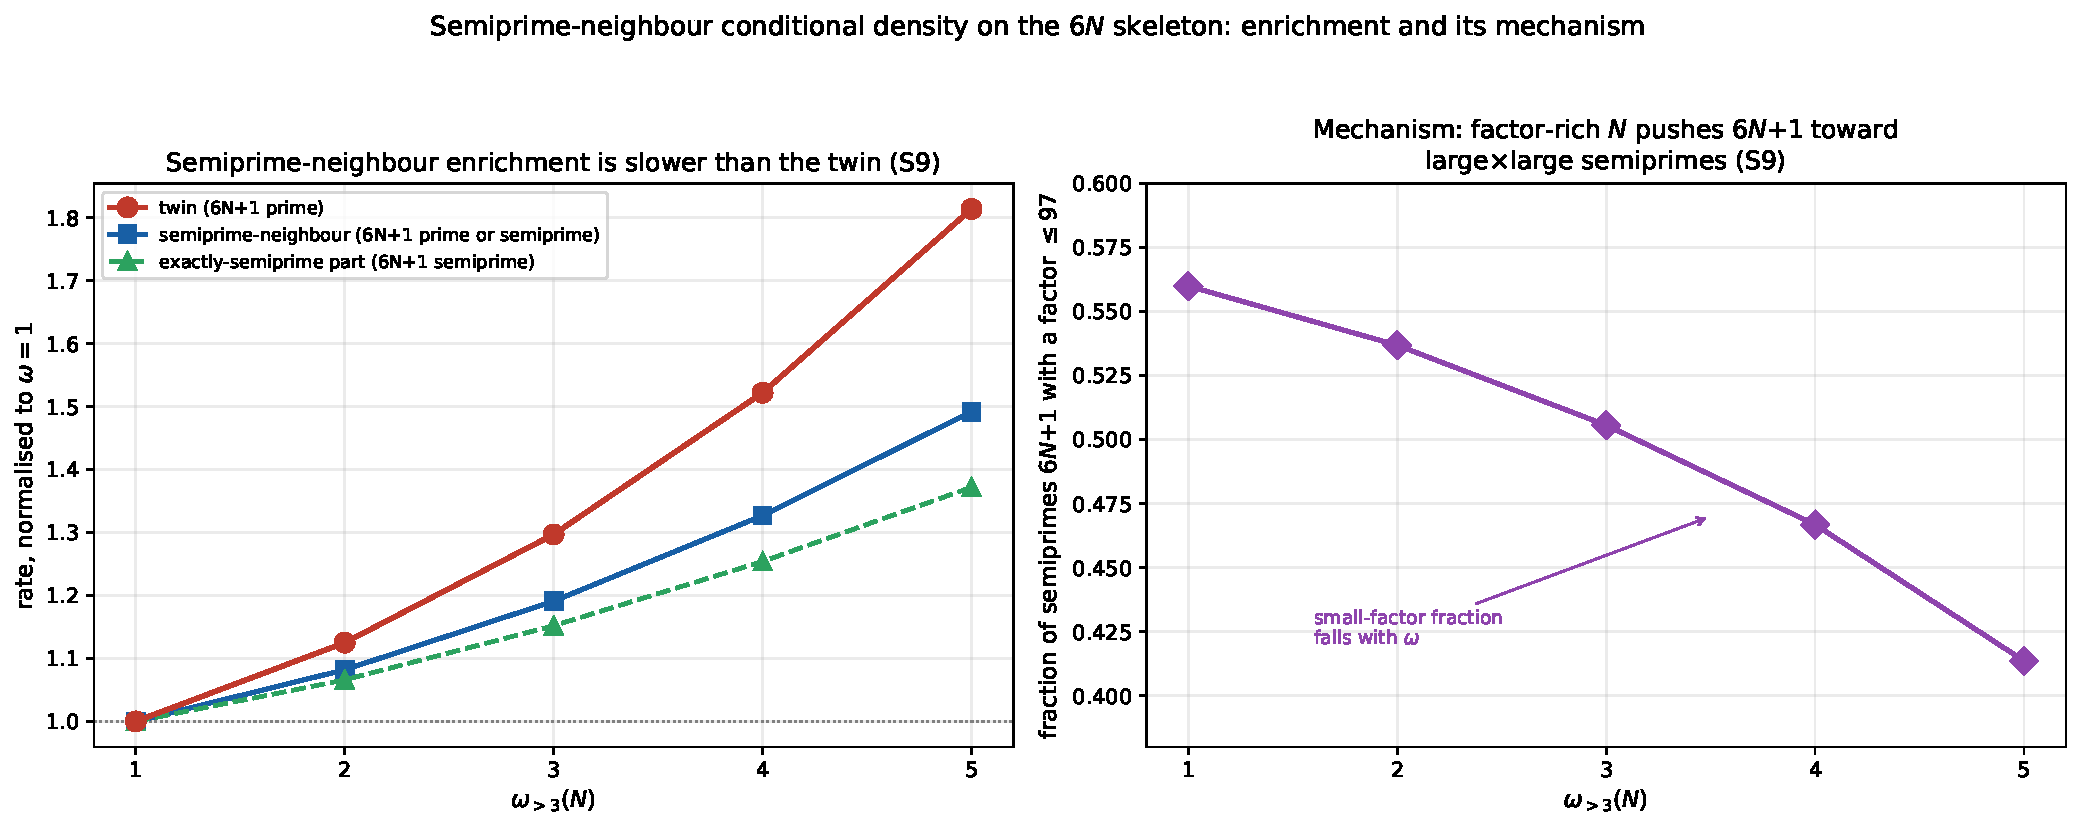
\includegraphics[width=\textwidth]{fig_paper16_semiprime.pdf}
\caption{Left ($S_9$): enrichment of the twin (fastest), the semiprime-neighbour
(intermediate), and the exactly-semiprime part (slowest). Right ($S_9$): among
semiprime $6N+1$, the fraction with a small prime factor ($\le97$) falls with
$\omega$ (from $0.56$ to $0.41$), confirming the shift toward large$\times$large semiprimes.}
\label{fig:semi}
\end{figure}

\section{Scope and the open closed form}

The single-prime and semiprime local densities are classical
(Hardy--Littlewood for the prime wing; Landau's semiprime density for the relaxed
wing); this paper introduces no new density formula. The contribution is the
measured fact that the semiprime neighbour enriches more slowly than the twin, and
the factor-structure mechanism for it, verified by the falling small-factor
fraction.

We do \emph{not} claim an exact closed form for the semiprime enrichment. The twin
enrichment reduces to the clean single-prime law $1/(q-2)$ (Part~XII), but the
semiprime condition $\Omega(6N+1)=2$ couples \emph{two} prime factors, and the
$\omega$-dependence does not separate into a single per-prime factor; a faithful
model would be a double-factor convolution that we find does not reduce to a clean
product at the percent level. We therefore report the enrichment and its mechanism
empirically and leave the exact double-factor closed form as an open problem,
rather than force an approximate product. As throughout this series, no statement
is made about the infinitude of twins, semiprime neighbours, or any pattern.

\section{Conclusion}

Relaxing the twin's right wing from prime to prime-or-semiprime yields a count that
still enriches with $\omega_{>3}(N)$ but more slowly---to $1.37\times$ at
$\omega=5$ for the exactly-semiprime part, against $1.81\times$ for the twin. The
mechanism is that a factor-rich $N$'s small-prime avoidance helps a prime more than
a semiprime, pushing surviving semiprimes toward large$\times$large products, which
we confirm directly. The exact double-factor closed form is left open. This places
the semiprime neighbour alongside the cousin and sexy pairs as a relaxation of the
twin whose conditional shape is set, qualitatively and mechanistically, by the same
small-prime factor structure.

\paragraph{Data and code availability.}
The enrichment counts and the small-factor diagnostic are openly
available~\cite{repo}.

\begin{thebibliography}{9}
\bibitem{ChenI} R.~Chen, \emph{Prime distribution on the $6N$ skeleton} (Part~I),
Zenodo, doi:10.5281/zenodo.20470367 (2026).
\bibitem{ChenXII} R.~Chen, \emph{The factor statistics of twin centres}
(Part~XII), Zenodo, doi:10.5281/zenodo.20528446 (2026).
\bibitem{Landau} E.~Landau, \emph{Handbuch der Lehre von der Verteilung der
Primzahlen}, Teubner, 1909 (semiprime density).
\bibitem{repo} R.~Chen, \emph{$6N$ semiprime neighbour: data and code},
\url{https://github.com/Ruqing1963/6N-semiprime-neighbour} (2026).
\end{thebibliography}

\end{document}
